% \chapter{Tests and Results}
\chapter{Rezultate teoretice și experimentale}
\label{cap:rezultate}
Comparația corectă a diferitelor algoritmi de segmentare semantică a imaginilor și de detecția obiectelor este o sarcină foarte grea; nu se poate stabili care dintre modele este cel mai bun. În aplicațiile din viața reală, alegerea modelului potrivit se face prin balansarea capabilităților ei: viteza de funcționare și acuratețe. Pe lângă alegerile referitoare la detector, câțiva alți factori trebuie luate în considerare când vorbim de comparație:

% enumerate shit which is crucial for making a good object detector
\begin{enumerate}
	\item rezoluția imaginii de intrare
	\item numărul propunerilor generate pentru a fi clasificate
	\item setul de antrenare
	\item extractorul de trăsături folosit
	\item funcția de cost pentru antrenare de localizare
	\item configurarea antrenării (viteza de antrenare a rețelei neuronale, mărimea loturilor de antrenare, micșorarea ratei de învățare)
	\item etc.
\end{enumerate}

Mai rău, technologia evoluează atât de repede încât orice comparație devine încechită destul de repede.\newline
În această parte a lucrării sumarizăm rezultatele din articole individuale, pentru a arăta imaginea de ansamblu a algoritmilor.

\section{Rezultate de Performanță}
În această secțiune sumarizăm performanțele diferitelor modele raportate în articolele corespunzătoare.\newline
Metrica pentru măsurarea performanței în contextul detecției obiectelor este \textit{mAP (mean Average Precision)}. Este definit ca \textit{the average of the maximum precisions at different recall values}, adică media maximelor precizii la diferite valori de rechemare. Pentru a înțelege acest concept, trebuie mai întâi să recapitulăm conceptele de precizie și rechemare mai întâi.
\paragraph{Precizie} măsoară acuratețea predicțiilor, i.e. procentul predicțiilor corecte.
\begin{equation}
Precizie = \frac{TruePositive}{TruePositive + FalsePositive}.
\end{equation}

\paragraph{Recall (rechemare)} măsoară cât de precise sunt identificările pozitive.
\begin{equation}
Recall = \frac{TruePositive}{TruePositive + FalsNegative}.
\end{equation}

\paragraph{AP} \textit{Average Precision} este media a mai multor IoU pentru toate categoriile de obiecte.

Următorul tabel prezintă preciziile diferitelor rețele de detectare de obiecte:

\begin{center}
    \begin{tabular}{| l | l | l | l |}
    \hline
    Method & mAP (\%) & lowest speed (fps) & highest speed (fps)\\ \hline
    Fast R-CNN & 75.9 & 3 & 7  \\ \hline
    Faster R-CNN & 75.9 & 5 & 17 \\ \hline
    R-FCN & 82.0 & 6 & 10  \\ \hline
    SSD & 81.6 &22 & 59 \\  \hline
    YOLO & 66.4 & 40 & 91 \\  \hline
    \end{tabular}
\end{center}

Referitor la acest tabel trebuie să ținem în minte că rezoluția imaginilor de intrare și extractorul de trăsături au impact asupra vitezei de funcționare a rețelelor. În acest table putem găsi extremitățile în ceea ce privește viteza diferitelor sisteme.\newline
Până aici putem observa că detectoarele \textit{single shot} au viteze impresive; articolele încearcă să dovedească că aceste modele au avantaj în precizie față de modelele bazate pe regiuni (R-CNN, Fast RCNN, etc). Diferite metode de optimizare sunt folosite de autori, astfel izolarea beneficiilor aduse de fiecare model devine foarte grea. Adevărul este că detectoarele \textit{single shot} și cele bazate pe clasificare de regiuni încep să devină similare în ceea ce privește designul. Ce putem să zicem este că:
\begin{enumerate}
	\item metodele bazate pe regiuni cum ar fi Faster R-CNN au un mic avantaj de acuratețe, și pot fi folositoare dacă nu este nevoie de detectare în timp real
	\item detectoarele \textit{single shot} sunt bune pentru procesare în timp real, sacrificând acuratețea. Aplicațiile din viața reală trebuie să verifice dacă acuratețea sistemului single shot este satisfăcătoare.
\end{enumerate}

\section{Teste de funcționalitate și de performanță}
În această secțiune se va prezenta cum am testat detectorul de obiecte YOLO v3. YOLO este un detector tip single shot, adică nu se generează regiuni cu potențial mare de a conține vreun obiect de interes, ci imaginea întreagă se evaluează o singură dată.\newline
Pentru a asambla un sistem funcțional cu detectorul YOLO v3, folosim PyTorch codul fiind compatibil cu Python 3.5 și PyTorch 0.4.\newline
YOLO are 75 de straturi convoluționale, fără niciun strat de pooling. Fiind o rețea complet convoluțională, dimensiunile imaginilor de intrare nu ne interesează, rețeaua fiind compatibilă cu orice format. Dar din motive technice, vom folosi imagini de dimensiune uniformă (pentru a ține rezultatele consistente, pentru antrenare paralelă pe batch-uri, etc.). De obicei trăsăturile învățate de straturile convoluționale sunt încărcate într-un clasificator care efectuează pasul de detectare. În YOLO predicția se face folosind straturi convoluționale de dimensiunea 1x1. În YOLO se poate face predicția pe diferite scale, adică mărimi de obiecte. Stratul de detecție este folosit pentru a detecta trăsăturile de pe trăsăturile extrase cu \textit{stride} diferit, și anume 32, 16, 8. Asta înseamnă că pentru o intrare de 416x416 facem detecții pe o scală de 13x13, de 26x26 și de 52x52. Pentru o imagine de intrare cu rezoluția specificată, YOLO genereaă $(52x52 + 26x26 + 13x13)x3$ predicții, adică 10647. Dacă imaginea de fapt conține un singur obiect de interes, atunci cumva trebuie să reducem 10647 regiuni în 1 pentru singurul obiect. Pentru această sarcină folosim NMS, adică \textit{non-maximum suppression}.\newline
Pentru testare vom folosi o rețea antrenată pe setul de antrenare Microsof COCO (Common Objects in Context), modelul fiind capabil de a recunoaște 80 clase diferite de obiecte. Ponderile rețelei antrenate pot fi descărcate online acestea în forma unui fișier binar. Citirea fișierului binar trebuie făcută cu mare grijă deoarece în fișier nu putem găsi nicio informație despre ponderi; fișierul conține numai o serie de numere floating point. Dacă din greșeală citim ponderea unui neuron dintr-un strat convoluțional și o încărcăm într-un strat batch norm, nimeni nu ne oprește.\newline
În acest moment sistemul este capabil să genereze Nx10647 de regiuni, N fiind numărul claselor de obiecte care ne interesează. Pentru a obține un bounding box per obiect folosim algoritmul non-maximum suppression.\newline
Pentru a rula codul pe o serie de imagini trebuie să facem următorii pași:
\begin{itemize}
\item încărcăm rețeaua (straturile, configurațiile straturilor, și legăturile dintre ele)
\item încărcăm ponderile modelului antrenat pe Microsoft COCO
\item citim imaginile de intrare (pentru încărcarea imaginilor folosim librăria OpenCV)
\item organizăm imaginile de testare într-o serie de batch-uri
\item creăm bucla de detectare de obiecte
\item desenăm dreptunghiurile generate de sistem pe imagine (bounding boxes)
\item printăm rezultatele
\end{itemize}

%object detection with YOLO
\begin{figure}[h!]
    	\centering
	\captionsetup{justification=centering, margin=2cm}
	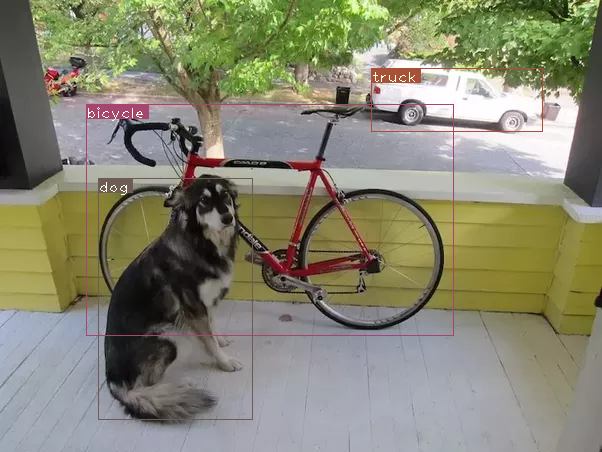
\includegraphics[width=0.8\textwidth]{figures/det_dog-cycle-car.png}
	\caption{Obiecte detectate \cite{DBLP:journals/corr/abs-1804-02767}}
	\label{fig:lethalities}
\end{figure}

\subsubsection{Rezultate}
Rezultatele produse de rețeaua asamblată mai sus sunt prezentate în tabela următoare. Prima coloană reprezintă mAP (mean Average Precision), adică media acurateței tuturor categoriilor de obiecte de interes, după care fiecare coloană reprezintă AP pentru clasa respectivă de obiecte.

\begin{table}[h]
\centering
$\begin{array}{ *{20}{c} }
\toprule
mAP & aero & bike  & bird   & boat & bottle & bus & car  & cat    & chair & cow  & table & dog  & horse\\
\midrule
73.2 & 86.3 & 81.5 & 73.6 & 58.7 & 51.7 & 79.9 & 77.0 & 90.6 & 51.8  & 78.2 & 58.5 & 89.2 & 82.4\\
\bottomrule
\end{array}$
\end{table}

Viteza medie a fost 23 imagini pe secundă (23 FPS), minimul fiind 10 iar maximul fiind 34. Numerele sunt mai mici decât cele prezentate de către Joseph Redmon et. al. în \cite{DBLP:journals/corr/abs-1804-02767} cauza fiind diferența dintre hardware-ul computerului care rulează programul.


\subsection{Viteză v.s. Acuratețe}
Întrabarea \textit{care detector este cel mai bun?} nu are răspuns corect, și nici nu este cea mai importantă întrebare; de fapt singurul lucru pe care putem să-l facem este să găsim cea mai bună soluție pentru un context anume. În fiecare situație trebuie să face un compromis între viteză și acuratețe, aceste două calități dorite fiind într-un trade-off.\newline
Putem să zicem însă că rețelele single-shot sunt cele mai rapide (SSD cu MobileNet având cea mai bună acuratețe dar funcționând foarte repede), iar metodele \textit{region based} satisfac cerința de acuratețe cu mai mult succes.